\documentclass{standalone}
\usepackage{xcolor}
\usepackage{verbatim}
\usepackage[T1]{fontenc}
\usepackage{graphics}
\usepackage{hyperref}
\newcommand{\code}[1]{\texttt{#1}}
\newcommand{\R}{R}
\newcommand{\pkg}[1]{#1}
\newcommand{\CRANpkg}[1]{\pkg{#1}}%
\newcommand{\BIOpkg}[1]{\pkg{#1}}
\usepackage{amsmath,amssymb,array}
\usepackage{booktabs}
\usepackage{multicol, calc}
\usepackage{tikz}
\usetikzlibrary{patterns,positioning,babel}
\usepackage{threeparttable}
\usepackage{natbib}
\usepackage{inconsolata}
\usepackage{listings}
\usepackage{tikz-qtree}
\usepackage{subcaption} 

\begin{document}
\nopagecolor
		
		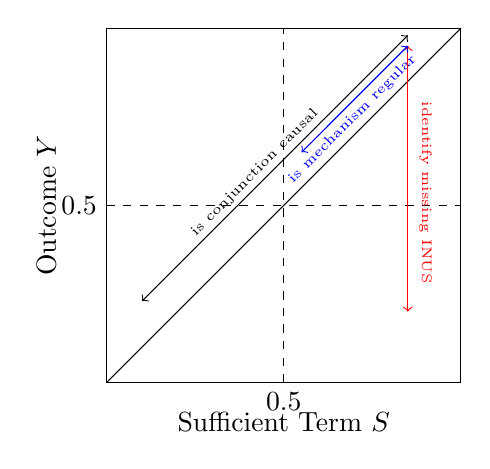
\begin{tikzpicture}[scale=4.5]
		\draw[black] (0,0) -- (1,0) node at (0.5,-0.11){Sufficient Term $S$};
		\draw[black] (0,0) -- (0,1) node at (-0.17,0.5)[rotate=90] {Outcome $Y$};
		\draw[black] (0,0) -- (1,1);
		\draw[black] (0,1) -- (1,1);
		\draw[black] (1,0) -- (1,1);
		\draw[dashed] (0.5,0) -- (0.5, 1);
		\draw[dashed] (0,0.5) -- (1, 0.5);
		\node[below] at (0.5,0){$0.5$};
		\node[left] at (0,0.5){$0.5$};
		%\node[above] at (0.65,0.85){\small typical};
		%\node[above] at (0.75,0.05){\small deviant cons};
		%\node[above] at (0.1,0.05){\small IIR};
		\node[right, rotate=45, blue] at (0.5,0.55){\tiny is mechanism regular};
		\draw[<->, red] (0.85, 0.95) -- (0.85, 0.2) ;
		\node[right, rotate=-90, red] at (0.9,0.82) {\tiny identify missing INUS};
		\draw[<->] (0.85, 0.98) -- (0.1, 0.23) ;
		\node[above, rotate=45] at (0.45,0.56) {\tiny is conjunction causal};
		\draw[<->, blue] (0.85, 0.95) -- (0.55, 0.65) ;
		\end{tikzpicture}
		\qquad
		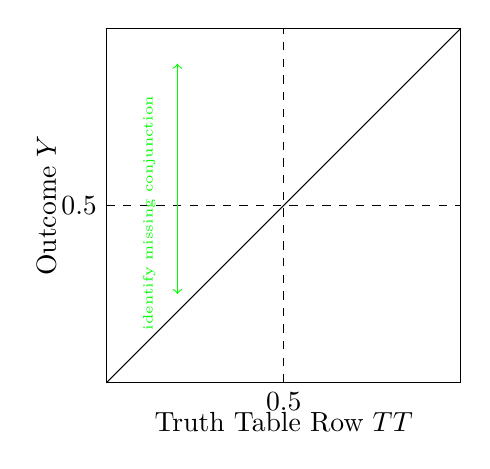
\begin{tikzpicture}[scale=4.5]
		\draw[black] (0,0) -- (1,0) node at (0.5,-0.11){Truth Table Row $TT$};
		\draw[black] (0,0) -- (0,1) node at (-0.17,0.5)[rotate=90] {Outcome $Y$};
		\draw[black] (0,0) -- (1,1);
		\draw[black] (0,1) -- (1,1);
		\draw[black] (1,0) -- (1,1);
		\draw[dashed] (0.5,0) -- (0.5, 1);
		\draw[dashed] (0,0.5) -- (1, 0.5);
		\draw[<->, green] (0.2,0.9) -- (0.2,0.25);
		\node[right, rotate=90, green] at (0.12,0.12) {\tiny identify missing conjunction};
		\node[below] at (0.5,0){$0.5$};
		\node[left] at (0,0.5){$0.5$};
		\end{tikzpicture}
\end{document}
